\documentclass[aspectratio=169,12pt]{beamer}
\usepackage[utf8]{inputenc}
\usepackage{amsmath, amssymb}
\usepackage{booktabs}
\usepackage{colortbl}
\usepackage{hyperref}
\usepackage{makecell}
\usepackage{ragged2e}
\usepackage{bytefield}
\usepackage{tikz}
\usetikzlibrary{arrows.meta, positioning, shapes.geometric, calc, tikzmark, shapes.misc}
\usepackage{tcolorbox}
\usepackage{pgfplots}
\pgfplotsset{compat=1.17}

\usetheme{Madrid}
\usecolortheme{default}

% Custom colors
\definecolor{mygreen}{RGB}{0,128,0}
\definecolor{myblue}{RGB}{0,0,255}
\definecolor{myred}{RGB}{255,0,0}

\title{Computer Structure}
\subtitle{236267}
\author{Lihu Rappoport}
\date{}

\begin{document}

\frame{\titlepage}

% Slide 2: General Course Information
\begin{frame}{General Course Information}
\begin{itemize}
    \item \textbf{Grade}
    \begin{itemize}
        \item 20\% : 3 exercises (all mandatory) תקף -- submission in pairs
        \item 80\% final exam
    \end{itemize}
    \item \textbf{Come to the lectures and to the tutorials !}
    \begin{itemize}
        \item The material for the exam includes \underline{all} that is taught during the lectures and the tutorials -- the foils do not contain everything
    \end{itemize}
    \item \textbf{Course web site}
    \begin{itemize}
        \item \url{http://webcourse.cs.technion.ac.il/236267/}
        \item Foils will be on the web several days before each lecture
    \end{itemize}
\end{itemize}
\end{frame}

% Slide 3: Class Focus
\begin{frame}{Class Focus}
\begin{itemize}
    \item \textbf{CPU}
    \begin{itemize}
        \item Introduction: performance, instruction set (RISC vs. CISC)
        \item Pipeline, hazards
        \item Branch prediction
        \item Out-of-order execution
    \end{itemize}
    \item \textbf{Memory Hierarchy}
    \begin{itemize}
        \item Cache and cache coherency
        \item Main memory
        \item Virtual Memory
    \end{itemize}
    \item \textbf{More topics}
    \begin{itemize}
        \item Multi-threading
        \item System
        \item Power considerations
    \end{itemize}
\end{itemize}
\end{frame}

% Slide 4: Personal Computer System
\begin{frame}{Personal Computer System}
\centering
% Placeholder for complex system diagram
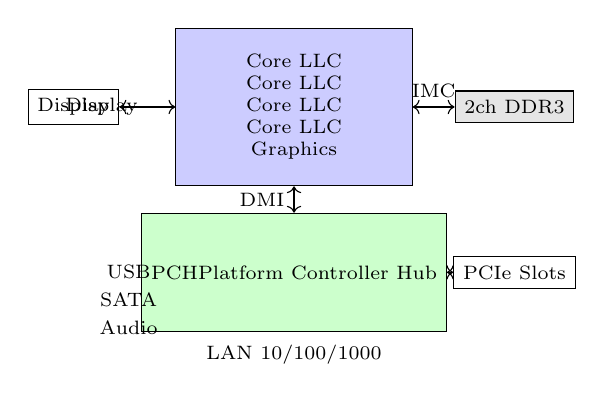
\begin{tikzpicture}[scale=0.7, every node/.style={font=\scriptsize}]
    % Note: This is a simplified version. Original has detailed PC architecture
    \node[draw, rectangle, fill=blue!20, minimum width=3cm, minimum height=2cm] (cpu) at (0,0) {
        \begin{tabular}{c}
            Core LLC\\
            Core LLC\\
            Core LLC\\
            Core LLC\\
            Graphics
        \end{tabular}
    };
    \node[draw, rectangle, fill=green!20, minimum width=2.5cm, minimum height=1.5cm] (pch) at (0,-3) {PCH\\Platform Controller Hub};
    \node[draw, rectangle, fill=gray!20] (memory) at (4,0) {2ch DDR3};
    \node[draw, rectangle] (display) at (-4,0) {Display};
    \node[draw, rectangle] (pcie) at (4,-3) {PCIe Slots};
    
    \draw[<->] (cpu) -- node[above] {IMC} (memory);
    \draw[<->] (cpu) -- node[left] {Display} (display);
    \draw[<->] (cpu) -- node[left] {DMI} (pch);
    \draw[<->] (pch) -- (pcie);
    
    % Peripherals
    \node at (-3,-3) {USB};
    \node at (-3,-3.5) {SATA};
    \node at (-3,-4) {Audio};
    \node at (0,-4.5) {LAN 10/100/1000};
\end{tikzpicture}

\vspace{0.5cm}
\textit{[Simplified diagram - full system architecture includes more components]}
\end{frame}

% Slide 5: Architecture & Microarchitecture
\begin{frame}{Architecture \& Microarchitecture}
\begin{itemize}
    \item \textbf{\textcolor{mygreen}{Architecture}}\\
    The processor features seen by the ``user''
    \begin{itemize}
        \item Instruction set, addressing modes, data width, \ldots
    \end{itemize}
    \vspace{0.3cm}
    \item \textbf{\textcolor{myblue}{Micro-architecture}}\\
    The internal implementation of a processor
    \begin{itemize}
        \item Caches size and structure, number of execution units, \ldots
    \end{itemize}
    \vspace{0.3cm}
    \item Processors with different $\mu$Arch can support the same architecture
    \vspace{0.3cm}
    \item \textbf{Compatibility}
    \begin{itemize}
        \item A new processor can run existing software
        \item The processor $\mu$Arch is new, but it supports the Architecture of past generations, possibly adding to it
    \end{itemize}
\end{itemize}
\end{frame}

% Slide 6: MOSFET Scaling
\begin{frame}{Moore's Law: Transistor Count Doubles Every Two Years}
\centering
\begin{tikzpicture}
    % Background: Transistor count PNG image - sized to fit frame
    \node[anchor=center, inner sep=0] (image) at (0,0) {
        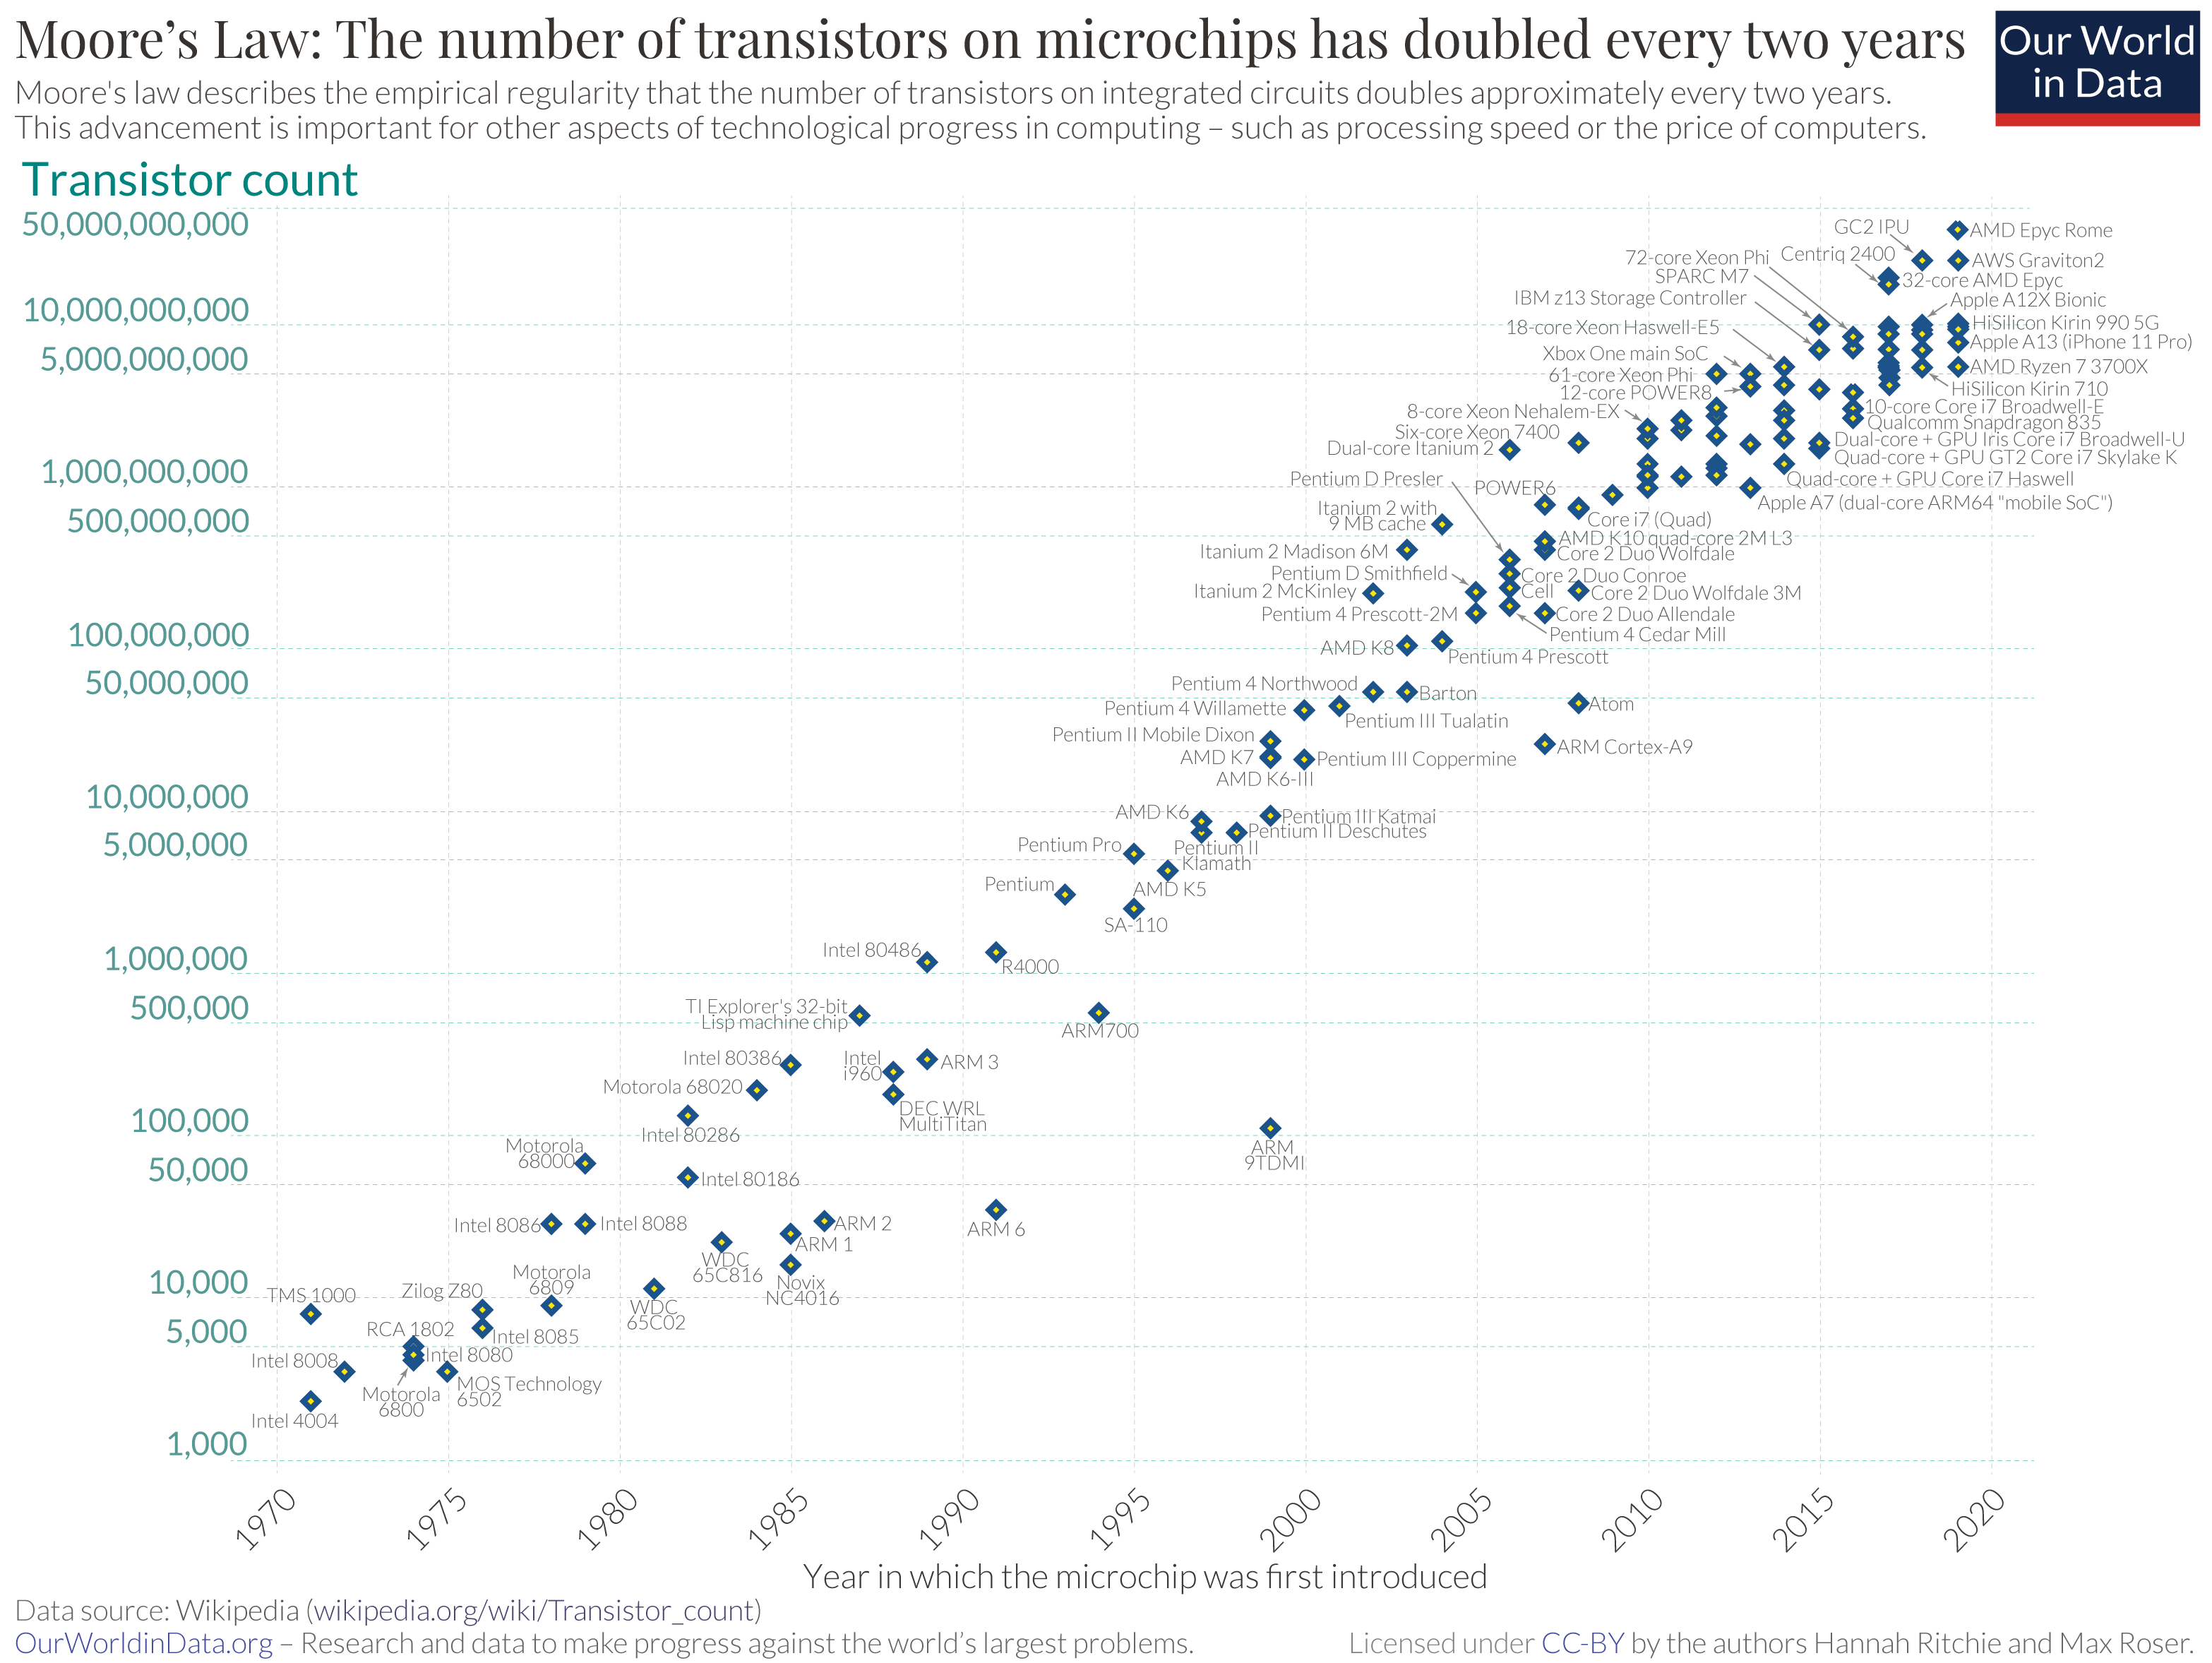
\includegraphics[width=\textwidth,height=0.75\textheight,keepaspectratio]{figures/Transistor-Count-over-time.png}
    };
    
    % Overlay: MOSFET scaling plot on top of the image - full width
    \begin{scope}
        \begin{semilogyaxis}[
            at={(image.south west)},
            anchor=south west,
            width=\textwidth,
            height=0.75\textheight,
            xmin=1970, xmax=2025,
            ymin=1, ymax=20000,
            hide x axis,
            hide y axis,
            legend pos=north east,
            legend style={font=\scriptsize, fill=white, fill opacity=0.8, draw=red!80!black},
            axis background/.style={fill=none}
        ]
        % MOSFET scaling data points with labels
        \addplot[
            red, 
            very thick, 
            mark=*, 
            mark size=2pt, 
            mark options={fill=red},
            nodes near coords,
            point meta=explicit symbolic,
            every node near coord/.append style={
                font=\tiny,
                text=red!80!black,
                anchor=south
            }
        ] coordinates {
            (1971, 10000) [10$\mu$m]
            (1974, 6000) [6$\mu$m]
            (1977, 3000) [3$\mu$m]
            (1981, 1500) [1.5$\mu$m]
            (1984, 1000) [1$\mu$m]
            (1987, 800) [800nm]
            (1990, 600) [600nm]
            (1993, 350) [350nm]
            (1996, 250) [250nm]
            (1999, 180) [180nm]
            (2001, 130) [130nm]
            (2003, 90) [90nm]
            (2005, 65) [65nm]
            (2007, 45) [45nm]
            (2009, 32) [32nm]
            (2012, 22) [22nm]
            (2014, 14) [14nm]
            (2016, 10) [10nm]
            (2018, 7) [7nm]
            (2020, 5) [5nm]
            (2022, 3) [3nm]
            (2025, 2) [2nm]
        };
        \addlegendentry{MOSFET Feature Size}
        \end{semilogyaxis}
    \end{scope}
\end{tikzpicture}
\end{frame}

% Slide 7: CPU Performance
\begin{frame}{CPU Performance}
\begin{itemize}
    \item \textbf{CPUs work according to a clock signal}
    \begin{itemize}
        \item Clock cycle is measured in nsec ($10^{-9}$ of a second)
        \item Clock frequency (= $\frac{1}{\text{clock cycle}}$) measured in GHz ($10^9$ cyc/sec)
    \end{itemize}
    \vspace{0.5cm}
    \item \textbf{CPI -- Cycles Per Instruction}
    \begin{itemize}
        \item Average \#cycles per Instruction (in a given program)
        \item IPC (= $\frac{1}{\text{CPI}}$) : Instructions per cycles
    \end{itemize}
\end{itemize}

\vspace{0.5cm}
\begin{center}
\Large
$$\text{CPI} = \frac{\text{Total number of cycles required to execute the program}}{\text{Total number of instructions executed in the program}}$$
\end{center}
\end{frame}

% Slide 8: Calculating the CPI of a Program
\begin{frame}{Calculating the CPI of a Program}
\begin{itemize}
    \item $IC_i$: \#times instruction of type $i$ is executed in the program
    \item IC: \#instruction executed in the program: $IC = \sum_{i=1}^{n} IC_i$
    \item $F_i$: relative frequency of instruction of type $i$: $F_i = \frac{IC_i}{IC}$
    \item $CPI_i$ -- \#cycles to execute instruction of type $i$
    \begin{itemize}
        \item e.g.: $CPI_{add} = 1$, $CPI_{mul} = 3$
    \end{itemize}
    \item \#cycles required to execute the entire program:
    $$\#cyc = \sum_{i=1}^{n} CPI_i \times IC_i = CPI \times IC$$
    \item CPI:
    $$CPI = \frac{\#cyc}{IC} = \frac{\sum_{i=1}^{n} CPI_i \times IC_i}{IC} = \sum_{i=1}^{n} CPI_i \times \frac{IC_i}{IC} = \sum_{i=1}^{n} CPI_i \times F_i$$
\end{itemize}
\end{frame}

% Slide 9: CPU Time
\begin{frame}{CPU Time}
\begin{itemize}
    \item \textbf{CPU Time} - time required to execute a program
    \begin{center}
    \Large
    \colorbox{yellow!20}{CPU Time = IC $\times$ CPI $\times$ clock cycle}
    \end{center}
    \vspace{0.5cm}
    \item \textbf{Our goal: minimize CPU Time}
    \begin{itemize}
        \item Minimize clock cycle: more GHz (process, circuit, uArch)
        \item Minimize CPI: \hspace{1.5cm} uArch (e.g.: more execution units)
        \item Minimize IC: \hspace{2cm} architecture (e.g.: vector instructions)
    \end{itemize}
\end{itemize}
\end{frame}

% Slide 10: Amdahl's Law
\begin{frame}{Amdahl's Law}
Suppose enhancement E accelerates a fraction F of the task by a factor S, and the remainder of the task is unaffected, then:

\vspace{0.3cm}
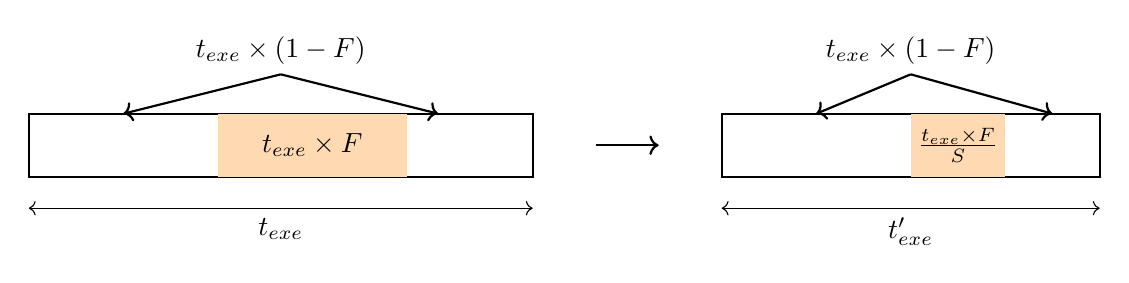
\begin{tikzpicture}[scale=0.8]
    % Original execution
    \draw[thick] (0,1) rectangle (8,2);
    \fill[orange!30] (3,1) rectangle (6,2);
    \node at (4.5,1.5) {$t_{exe} \times F$};
    \draw[<->] (0,0.5) -- (8,0.5) node[midway, below] {$t_{exe}$};
    
    % Label for (1-F) parts with arrows
    \node (label1) at (4,3) {$t_{exe} \times (1-F)$};
    \draw[->, thick] (label1.south) -- (1.5,2);
    \draw[->, thick] (label1.south) -- (6.5,2);
    
    % Arrow
    \draw[->, thick] (9,1.5) -- (10,1.5);
    
    % Enhanced execution
    \draw[thick] (11,1) rectangle (17,2);
    \fill[orange!30] (14,1) rectangle (15.5,2);
    \node at (14.75,1.5) {$\frac{t_{exe} \times F}{S}$};
    \draw[<->] (11,0.5) -- (17,0.5) node[midway, below] {$t'_{exe}$};
    
    % Label for (1-F) parts with arrows
    \node (label2) at (14,3) {$t_{exe} \times (1-F)$};
    \draw[->, thick] (label2.south) -- (12.5,2);
    \draw[->, thick] (label2.south) -- (16.25,2);
\end{tikzpicture}

\vspace{0.5cm}
$$t'_{exe} = t_{exe} \times \left[(1-F) + \frac{F}{S}\right]$$

$$\text{Speedup}_{overall} = \frac{t_{exe} - t'_{exe}}{t_{exe}} = 1 - \left[(1-F) + \frac{F}{S}\right] = F - \frac{F}{S}$$
\end{frame}

% Slide 11: Amdahl's Law Example
\begin{frame}{Amdahl's Law: Example}
\begin{itemize}
    \item Floating point instructions improved to run 2$\times$ faster
    \item 10\% of the executed instructions are FP instruction
\end{itemize}

\vspace{0.5cm}
$$t'_{exe} = t_{exe} \times (0.9 + 0.1 / 2) = 0.95 \times t_{exe}$$

$$\text{Speedup}_{overall} = 1 - 0.95 = 0.05 = 5\%$$

\vspace{1cm}
\begin{center}
\colorbox{gray!20}{
\Large Corollary: Make The Common Case Fast
}
\end{center}
\end{frame}

% Slide 12: Evaluating Performance of future CPUs
\begin{frame}{Evaluating Performance of future CPUs}
\begin{itemize}
    \item \textbf{Use a performance simulator to evaluate the performance of a new feature / algorithm}
    \begin{itemize}
        \item Models the uarch to a great detail
        \item Run 100's of representative applications
    \end{itemize}
    \item \textbf{Produce the performance s-curve}
    \begin{itemize}
        \item Sort the applications according to the IPC increase
        \item Baseline (0) is the processor without the new feature
    \end{itemize}
\end{itemize}

\begin{columns}
\column{0.5\textwidth}
\centering
\textbf{S-curve with negative results}\\
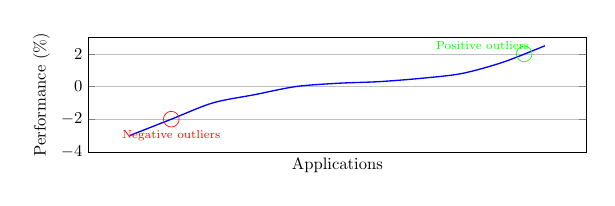
\begin{tikzpicture}[scale=0.6]
    \begin{axis}[
        xlabel={Applications},
        ylabel={Performance (\%)},
        width=\textwidth,
        height=4cm,
        ymin=-4, ymax=3,
        grid=major,
        xtick=\empty
    ]
    \addplot[blue, thick, smooth] coordinates {
        (0,-3) (10,-2) (20,-1) (30,-0.5) (40,0) (50,0.2) 
        (60,0.3) (70,0.5) (80,0.8) (90,1.5) (100,2.5)
    };
    \node[red, circle, draw] at (axis cs:10,-2) {};
    \node[red] at (axis cs:10,-3) {\scriptsize Negative outliers};
    \node[green, circle, draw] at (axis cs:95,2) {};
    \node[green] at (axis cs:85,2.5) {\scriptsize Positive outliers};
    \end{axis}
\end{tikzpicture}

\column{0.5\textwidth}
\centering
\textbf{S-curve of a good feature}\\
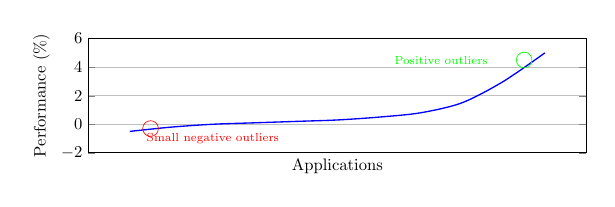
\begin{tikzpicture}[scale=0.6]
    \begin{axis}[
        xlabel={Applications},
        ylabel={Performance (\%)},
        width=\textwidth,
        height=4cm,
        ymin=-2, ymax=6,
        grid=major,
        xtick=\empty
    ]
    \addplot[blue, thick, smooth] coordinates {
        (0,-0.5) (10,-0.2) (20,0) (30,0.1) (40,0.2) (50,0.3) 
        (60,0.5) (70,0.8) (80,1.5) (90,3) (100,5)
    };
    \node[red, circle, draw] at (axis cs:5,-0.3) {};
    \node[red] at (axis cs:20,-1) {\scriptsize Small negative outliers};
    \node[green, circle, draw] at (axis cs:95,4.5) {};
    \node[green] at (axis cs:75,4.5) {\scriptsize Positive outliers};
    \end{axis}
\end{tikzpicture}
\end{columns}
\end{frame}

% Slide 13: Using Benchmarks for Comparing Performance
\begin{frame}{Using Benchmarks for Comparing Performance}
\begin{itemize}
    \item \textbf{Benchmark types}
    \begin{itemize}
        \item Real applications, or representative parts of real apps
        \item Synthetic benchmarks which represent typical workloads
    \end{itemize}
    \vspace{0.3cm}
    \item \textbf{Benchmarks are targeted at the specific system usages}
    \begin{itemize}
        \item \textbf{SPEC INT} -- integer applications: data compression, C compiler, Perl interpreter, database system, chess-playing, Text-processing, \ldots
        \item \textbf{SPEC FP} -- floating point applications: fluid dynamics, quantum chemistry, image ray-tracing, speech recognition, \ldots
        \item \textbf{SYSMark} -- reflects usage patterns of business users
        \begin{itemize}
            \item office productivity: Acrobat, Excel, PowerPoint, Word
            \item media creation: Photoshop, Premiere, Sketchup
            \item data/financial analysis: Excel, WinZip
        \end{itemize}
        \item \textbf{TPC Benchmarks} - transaction-processing throughput
    \end{itemize}
\end{itemize}
\end{frame}

% Slide 14: Instruction Set Design
\begin{frame}{Instruction Set Design}
\centering
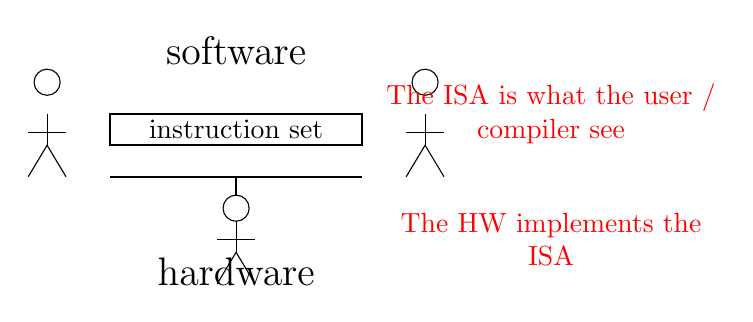
\begin{tikzpicture}[scale=0.8]
    % Software layer
    \node at (0,4) {\Large software};
    \draw[thick] (-2,3) -- (2,3);
    \draw[thick] (-2,2.5) rectangle (2,3);
    \node at (0,2.75) {instruction set};
    \draw[thick] (-2,2) -- (2,2);
    
    % Hardware layer
    \node at (0,0.5) {\Large hardware};
    
    % People
    \node[circle,draw] (user1) at (-3,3.5) {};
    \draw (-3,3) -- (-3,2.5);
    \draw (-3.3,2.7) -- (-2.7,2.7);
    \draw (-3.3,2) -- (-3,2.5) -- (-2.7,2);
    
    \node[circle,draw] (user2) at (3,3.5) {};
    \draw (3,3) -- (3,2.5);
    \draw (2.7,2.7) -- (3.3,2.7);
    \draw (2.7,2) -- (3,2.5) -- (3.3,2);
    
    % Hardware person
    \node[circle,draw] (hw) at (0,1.5) {};
    \draw (0,1.3) -- (0,0.8);
    \draw (-0.3,1) -- (0.3,1);
    \draw (-0.3,0.3) -- (0,0.8) -- (0.3,0.3);
    \draw[thick] (hw) -- (0,2);
    
    % Annotations
    \node[red, align=center] at (5,3) {The ISA is what the user /\\compiler see};
    \node[red, align=center] at (5,1) {The HW implements the\\ISA};
\end{tikzpicture}
\end{frame}

% Slide 15: ISA Considerations
\begin{frame}{ISA Considerations}
\begin{itemize}
    \item \textbf{Reduce the IC to reduce execution time}
    \begin{itemize}
        \item A single vector instruction performs the work of multiple scalar instructions
    \end{itemize}
    \vspace{0.3cm}
    \item \textbf{Simple instructions $\Rightarrow$ simpler HW implementation}
    \begin{itemize}
        \item Higher frequency, lower power, lower cost
    \end{itemize}
    \vspace{0.3cm}
    \item \textbf{Code size}
    \begin{itemize}
        \item Long instructions take more time to fetch and require a larger memory
        \begin{itemize}
            \item Important for large code footprint workloads
        \end{itemize}
    \end{itemize}
\end{itemize}
\end{frame}

% Slide 16: Architectural Consideration Example
\begin{frame}{Architectural Consideration Example}
\begin{itemize}
    \item \textbf{Most instructions use a short immediate value}
    \begin{itemize}
        \item Having all instructions support the maximum size needed would increase code size
    \end{itemize}
\end{itemize}

\centering
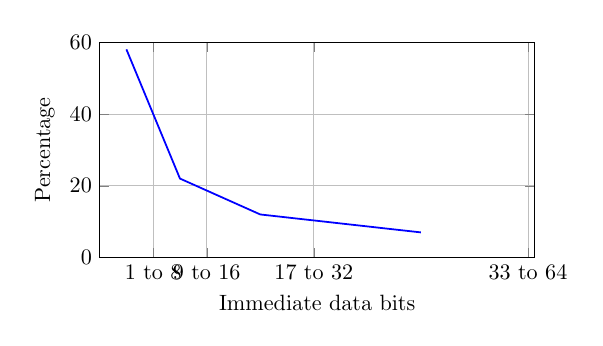
\begin{tikzpicture}[scale=0.8]
    \begin{axis}[
        xlabel={Immediate data bits},
        ylabel={Percentage},
        width=0.7\textwidth,
        height=5cm,
        ymin=0, ymax=60,
        xmin=0, xmax=65,
        xtick={8,16,32,64},
        xticklabels={1 to 8, 9 to 16, 17 to 32, 33 to 64},
        grid=major,
        bar width=15pt
    ]
    \addplot[blue, thick] coordinates {
        (4,58) (12,22) (24,12) (48,7)
    };
    \end{axis}
\end{tikzpicture}
\end{frame}

% Slide 17: ISA Extensions for Reducing IC
\begin{frame}{ISA Extensions for Reducing IC}
\textbf{Example}
\begin{itemize}
    \item 128-bit packed (vector) / scalar single precision FP (4×32)
    \item 128-bit registers (XMM0 -- XMM7)
\end{itemize}

\begin{columns}
\column{0.5\textwidth}
\centering
\textbf{Packed:}\\[0.3cm]
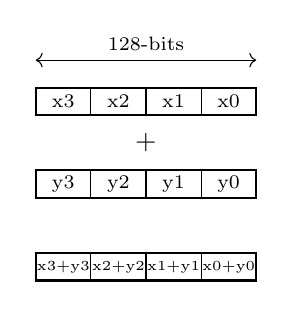
\begin{tikzpicture}[scale=0.7]
    \draw[thick] (0,2) rectangle (4,2.5);
    \foreach \x in {1,2,3} {
        \draw (\x,2) -- (\x,2.5);
    }
    \node at (0.5,2.25) {\scriptsize x3};
    \node at (1.5,2.25) {\scriptsize x2};
    \node at (2.5,2.25) {\scriptsize x1};
    \node at (3.5,2.25) {\scriptsize x0};
    
    \node at (2,1.5) {+};
    
    \draw[thick] (0,0.5) rectangle (4,1);
    \foreach \x in {1,2,3} {
        \draw (\x,0.5) -- (\x,1);
    }
    \node at (0.5,0.75) {\scriptsize y3};
    \node at (1.5,0.75) {\scriptsize y2};
    \node at (2.5,0.75) {\scriptsize y1};
    \node at (3.5,0.75) {\scriptsize y0};
    
    \draw[thick] (0,-1) rectangle (4,-0.5);
    \foreach \x in {1,2,3} {
        \draw (\x,-1) -- (\x,-0.5);
    }
    \node at (0.5,-0.75) {\tiny x3+y3};
    \node at (1.5,-0.75) {\tiny x2+y2};
    \node at (2.5,-0.75) {\tiny x1+y1};
    \node at (3.5,-0.75) {\tiny x0+y0};
    
    \draw[<->] (0,3) -- (4,3) node[midway, above] {\scriptsize 128-bits};
\end{tikzpicture}

\column{0.5\textwidth}
\centering
\textbf{Scalar:}\\[0.3cm]
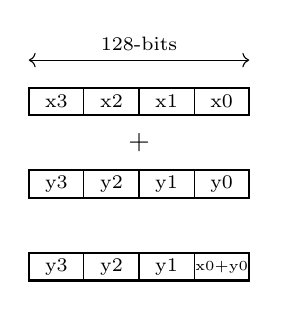
\begin{tikzpicture}[scale=0.7]
    \draw[thick] (0,2) rectangle (4,2.5);
    \foreach \x in {1,2,3} {
        \draw (\x,2) -- (\x,2.5);
    }
    \node at (0.5,2.25) {\scriptsize x3};
    \node at (1.5,2.25) {\scriptsize x2};
    \node at (2.5,2.25) {\scriptsize x1};
    \node at (3.5,2.25) {\scriptsize x0};
    
    \node at (2,1.5) {+};
    
    \draw[thick] (0,0.5) rectangle (4,1);
    \foreach \x in {1,2,3} {
        \draw (\x,0.5) -- (\x,1);
    }
    \node at (0.5,0.75) {\scriptsize y3};
    \node at (1.5,0.75) {\scriptsize y2};
    \node at (2.5,0.75) {\scriptsize y1};
    \node at (3.5,0.75) {\scriptsize y0};
    
    \draw[thick] (0,-1) rectangle (4,-0.5);
    \foreach \x in {1,2,3} {
        \draw (\x,-1) -- (\x,-0.5);
    }
    \node at (0.5,-0.75) {\scriptsize y3};
    \node at (1.5,-0.75) {\scriptsize y2};
    \node at (2.5,-0.75) {\scriptsize y1};
    \node at (3.5,-0.75) {\tiny x0+y0};
    
    \draw[<->] (0,3) -- (4,3) node[midway, above] {\scriptsize 128-bits};
\end{tikzpicture}
\end{columns}

\vspace{0.5cm}
\begin{itemize}
    \item A single ``packed add'' instruction replaces 4 ``add'' instructions
    \item In order to fully gain the performance, need also new HW
    \begin{itemize}
        \item execution unit that performs ``packed add'' in a single cycle
    \end{itemize}
\end{itemize}
\end{frame}

% Slide 18: CISC Processors
\begin{frame}[fragile]{CISC Processors}
\begin{itemize}
    \item \textbf{CISC -- Complex Instruction Set Computer} -- a high-level machine language
    \begin{itemize}
        \item Example: x86
    \end{itemize}
    \item \textbf{Complex instructions and complex addressing modes}\\
    $\Rightarrow$ complicates the processor and slows down the simple, common instructions\\
    $\Rightarrow$ contradicts \textcolor{red}{Make The Common Case Fast}
    \item \textbf{Small number of registers} $\Rightarrow$ requires many memory accesses
    \item \textbf{Non-orthogonal registers}: some operations supported only on specific registers\\
    $\Rightarrow$ Not compiler friendly
    \item \textbf{ALU operations directly on memory}
    \begin{verbatim}
    add  eax, 7680[ecx] ;eax ← MEM[7680+ecx]+ eax
    \end{verbatim}
    \item \textbf{Variable length instructions}
    \begin{itemize}
        \item Common instructions get short codes $\Rightarrow$ save code length
        \item Difficult to decode few instructions in parallel: only after an instruction is decoded, its length (and when the next instruction starts) is known
        \item An instruction may cross a cache line or a page
    \end{itemize}
\end{itemize}
\end{frame}

% Slide 19: Top 10 Instructions
\begin{frame}{Top 10 Instructions}
\centering
\begin{table}
\begin{tabular}{clr}
\toprule
\textbf{Rank} & \textbf{instruction} & \textbf{\% of total executed} \\
\midrule
1 & load & 22\% \\
2 & conditional branch & 20\% \\
3 & compare & 16\% \\
4 & store & 12\% \\
5 & add & 8\% \\
6 & and & 6\% \\
7 & sub & 5\% \\
8 & move register-register & 4\% \\
9 & call & 1\% \\
10 & return & 1\% \\
\midrule
& \textbf{Total} & \textbf{96\%} \\
\bottomrule
\end{tabular}
\end{table}

\vspace{0.5cm}
\Large
\textcolor{red}{Simple instructions dominate instruction frequency}
\end{frame}

% Slide 20: RISC Processors
\begin{frame}{RISC Processors}
\begin{itemize}
    \item \textbf{RISC -- Reduced Instruction Set Computer}
    \begin{itemize}
        \item Simple instructions enable fast hardware: make the common case fast
        \item Example: ARM
    \end{itemize}
    \item \textbf{Characteristics}
    \begin{itemize}
        \item A small instruction set, with few instruction formats
        \item Simple instructions that execute simple tasks, most of them single-cycle (with pipeline)
        \item A few addressing methods, with ALU operations on registers only
        \begin{itemize}
            \item Memory is accessed using Load and Store instructions only
        \end{itemize}
        \item Many orthogonal registers -- all instructions available with all registers
        \item Three address machine: \quad \texttt{add dst, src1, src2}
        \item Fixed length instructions
        \item Compiler friendly -- easier to utilize the ISA: orthogonal, simple
    \end{itemize}
\end{itemize}
\end{frame}

% Slide 21: RISC Processors (Cont.)
\begin{frame}{RISC Processors (Cont.)}
\begin{itemize}
    \item \textbf{Simple architecture $\Rightarrow$ Simple micro-architecture}
    \begin{itemize}
        \item Simple, small and fast control logic
        \item Simpler to design and validate
        \item Leave space for large on die caches
        \item Shorter time-to-market
    \end{itemize}
    \vspace{0.3cm}
    \item \textbf{Existing RISC processor are not ``pure'' RISC}
    \begin{itemize}
        \item E.g., support division which takes many cycles
    \end{itemize}
    \vspace{0.3cm}
    \item \textbf{Modern CISC processors use RISC $\mu$-arch ideas}
    \begin{itemize}
        \item Internally translate the CISC instructions into RISC-like operations
        \begin{itemize}
            \item the inside core looks much like that of a RISC processor
        \end{itemize}
    \end{itemize}
\end{itemize}
\end{frame}

\end{document}